Les processus de maintenance SPIE et SAP sont similaires sur de nombreux points. \\

Néanmoins, le choix de SAP a été de rendre indépendants les processus de gestion des contrats clients permettant de créer et de gérer les contrats relatifs aux services, et les processus de service et de réparation permettant au Service Client d’assurer des services de réparation et de maintenance. \\

Chez SPIE, cela correspond à une séparation des processus visant à créer et valider la commande et à créer le contrat (Offre et revue d’offre, Négociation client, Revue de commande), et des processus d’exécution des services de maintenance (Lancement, Réalisation, Évolution du contrat, Solde de l’affaire et du contrat). Le scénario de vente et gestion des contrats SAP, plus générique, permet de gérer tous les aspects du contrat, depuis la création à la facturation, en passant par la prestation de services, le renouvellement et l’annulation, et la cohérence financière. \\

En ce qui concerne les opérations de maintenance, le scénario SAP comporte un processus de confirmation d’exécution d’un service, qui permet de faire un reporting détaillé des opérations de maintenance effectuées chez le client . Cela sert à enregistrer des informations supplémentaires sur le travail exécuté, les causes profondes des problèmes causés par le produits, ou encore des feedbacks afin d’améliorer leur qualité. Cette phase est plus réduite dans le processus SPIE, ce qui rend l’accès au reporting plus difficile pour les techniciens. \\

Le sous-processus SPIE "Lancement des prestations de service et travaux" ne traite pas les achats de pièces nécessaires pour la maintenance, contrairement au scénario SAP, qui comprend des fonctions de gestion des domaines liés supportant directement les prestations de service, telles que le stockage et l’inventaire des pièces de rechange. Il peut être utile "destandardiser" cette phase du sous-processus de lancement afin d’estimer plus précisément les recettes de prestation. \\

Nous conseillons donc à SPIE d’inclure le processus \bf{Demande de résolution des contrats} pour pallier à cet éventuel manque que nous avons constaté dans les processus. \\

\begin{figure}[H]
    \label{fig-gestion-contrats-client}
    \noindent\makebox[\textwidth]{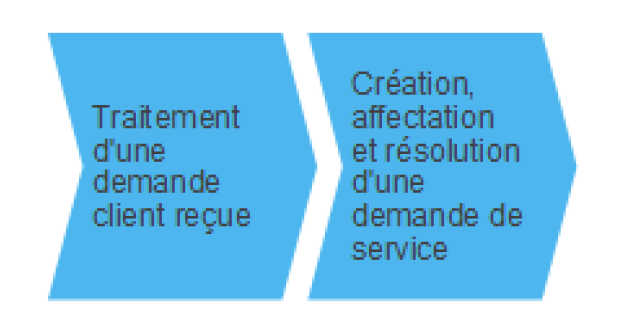
\includegraphics[width=5cm]{figures/demande_resolution_contrats.png}}
    \caption{Demande de résolution des contrats}
\end{figure}

Ce processus démarre lorsqu’un client appelle ou envoie un email pour signaler un problème avec un produit ou un service. Après réception de la demande, un agent du centre de service crée une demande de service. L’agent parcours alors la base de connaissance pour trouver une solution qui conviendrait à la résolution du problème. S’il en trouve une, il l’envoie au client et finalise la demande de service.
